\documentclass[]{auvsi_doc}
\setkeys{auvsi_doc.cls}{
	AUVSITitle={Bill of Materials},
	AUVSILogoPath={./../logo.pdf}
}

% include extra packages, if needed
\usepackage{tabularx}
\usepackage{booktabs}
\usepackage{longtable}

\begin{document}
	
	\begin{AUVSITitlePage}
		\begin{artifacttable}
			\entry{BM-001, 0.1, 02-19-2019, SS Engineering Draft, Ryan Anderson, CHECKED BY}
			% additional \entry{} commands for extra rows in the revision table, if needed
		\end{artifacttable}
	\end{AUVSITitlePage}
	
	% document contents (see below for LaTex commands that make your life easier)
	\section{Introduction}
	This artifact is meant to communicate the spatial layout of components in the plane. Note that only components with significant spacial requirements are included. This includes center of gravity, signal interference, and physical volume. A diagram of the current configuration is included in Fig. \ref{fig:components}.
	
	%Begin table
	
	\begin{table}[h!]
		\begin{center}
			\caption{Layout of components for ideal CG placement, avoiding signal interference, and practicality.}
			\label{table:components}
			\begin{tabular}{p{1cm}p{2.5cm}p{4cm}p{7cm}}
				\toprule
				Item \# & X Location (cm) & Item Description & Reason for Location & \\
				\midrule
				1 & 7.5 & GPS Antenna & Avoid interference with 5Ghz antenna \\
				2 & 17.5 & Ubiquiti Bullet & CG placement \\
				3 & 21.5 & Battery & CG placement \\
				4 & 33.5 & Camera & Near CG to reduce oscillations during image capture \\
				5 & 43.5 & Flight Controller and Inertial Sense & Inertial Sense should be near the CG  \\
				6 & 43.5 & Odroid & Central location is convenient for \newline connecting components \\
				7 & 52.5 & RC Antenna/Receiver & CG placement \\
				8 & 60.5 & UGV & CG placement, bay door design \\
				9 & 63 & 5GHz antenna & Avoid interference with GPS antenna \\
				10 & 68.5 & Parachute & Effective deployment with UGV \\
				\bottomrule
			\end{tabular}
		\end{center}
	\end{table}
	
	\begin{figure}[h!]
		\centering
		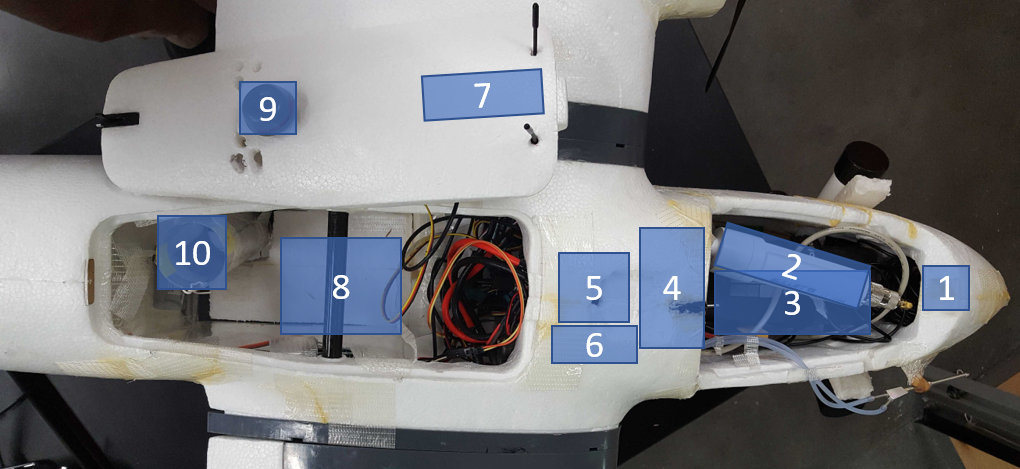
\includegraphics[width=.9\columnwidth]{figs/ComponentsPlacement.png}
		\caption{Diagram illustrating component placement.}
		\label{fig:components}
	\end{figure}
	
	
\end{document}
